\chapter{LDA+$U$和GW近似}
\section{LDA+$U$方法}
由于带电粒子间的\textrm{Coulomb}作用,运动中的电子间必然存在相互排斥。但是传统的能带理论为简化问题,处理电子系统时采用的是单粒子图像(平均场近似)。基于\textrm{DFT}理论虽然通过引入电子交换-相关泛函来修正电子间的相互作用,但由于精确的交换-相关泛函的形式未知,所以如何更好地描述电子关联(electron correlation)是伴随着\textrm{DFT}与生俱来的重要问题。\textrm{Perdew}的研究表明LDA近似和精确密度泛函方法的重要差别\cite{PRL49-1691_1982}:~尽管交换-相关泛函的精确形式不知,但总能量泛函对电子数的依赖$E(N)$应该具有折线特征(见图\ref{exact-DFT}):~
	\begin{displaymath}
		\dfrac{\Delta E}{\Delta N}=\left\{
		\begin{aligned}
			E(M)-E(M-1)|_{\mathrm{left}}\qquad M-1<N<M\\
			E(M+1)-E(M)|_{\mathrm{right}}\qquad M<N<M+1 
		\end{aligned}\right.
	\end{displaymath}
换句话说,电子数$N$改变整数值的时候,精确的单电子势$V(\vec r)=\dfrac{\delta E}{\delta n(\vec r)}$的改变应该是不连续的。而LDA近似下,显然势能是电子数$N$的连续函数。因为不具备势能随电子数变化不连续的特征,所以LDA方法在描述含有{\textit d}\,或{\textit f}\,电子的过渡金属和稀土元素化合物体系时常常失效。

\begin{figure}[h!]
\centering
\vspace*{-0.4in}
\includegraphics[height=2.4in,width=2.8in,viewport=0 0 1000 880,clip]{exact-DFT.png}
\caption{\small \textrm{The dependence of the total energy on the number of electron is a series of straight-line segments.}}%(与文献\cite{EPJB33-47_2003}图1对比)
\label{exact-DFT}
\end{figure}

Gunnarsson和Schonhammer\cite{PRL56-1968_1986}证明,单电子势的不连续对能带的带隙有很大的贡献。LDA近似的另一个不足还在于,LDA计算得到的轨道能量(定义为能量$E$对轨道占据数$n_i$的导数,即$\varepsilon_i=\partial E/\partial n_i$),不满足\textrm{Koopmans}定理,与实验或者严格计算得到的轨道能量差别很大。但是另一方面,LDA方法得到的总能量一般与实验结果符合的较好。一个典型的例子就是\textrm{H}原子的计算,LDA计算的轨道能为$-0.54\,\mathrm{Ry}$(实际结果为$-1.0\,\mathrm{Ry}$),总能量($-0.976\,\mathrm{Ry}$)则非常接近$-1.0\,\mathrm{Ry}$\cite{PRB37-9919_1988}。文献\inlinecite{PRB44-943_1991}提出通过对LDA势加入轨道校正克服LDA方法的不足(称为LDA+$U$方法)。LDA+$U$方法与\textrm{Andersen}掺杂模型\cite{PR124-41_1961}思想相同,对局域的{\textit d}\,或{\textit f}\,电子,采用模型Hamiltonian方法考虑$d$-$d$或$f$-$f$间相互作用(定域Coulomb相互作用$U$),离域的{\textit s}\,和{\textit p}\,电子的运动用LDA近似描述。

在文献\inlinecite{Herring}中,\textrm{Herring}讨论了$U$值的物理意义:~含有$n$个3{\textit d}\,电子的原子中,如果定义两个原子间转移一个{\textit d}\,电子,即
$$2(d^n)\rightarrow d^{n+1}+d^{n-1}$$
能量的改变为$U$
$$U=E(d^{n+1})+E(d^{n-1})-2E(d^n)$$
在\textrm{DFT}框架下,\textrm{L(S)DA}是弱耦合的平均场(\textrm{mean-filed, MF})理论,对于{\textit d}\,电子数目发生变化的原子/离子体系,$d$-$d$电子间的相互作用可以表示为$E=UN(N-1)/2$\cite{PRB48-16929_1993},将总能量中扣除LDA的$d$-$d$电子相互作用,再加上局域的电子间相互作用,可有
\begin{equation}
  E=E_{LDA}-UN(N-1)/2+\frac12U\sum_{i\neq j}n_in_j
  \label{eq:solid-251}
\end{equation}
由式\eqref{eq:solid-251}对轨道占据数$n_i$求导得轨道能
\begin{equation}
  \varepsilon_i=\frac{\partial E}{\partial n_i}=E_{LDA}+U(\frac12-n_i)
  \label{eq:solid-252}
\end{equation}
\begin{figure}[h!]
\centering
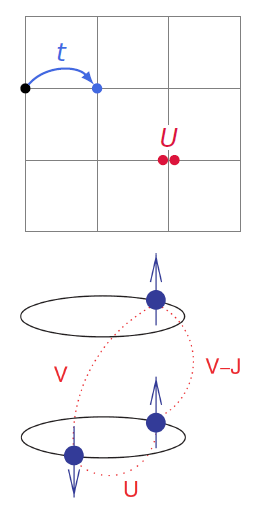
\includegraphics[height=1.35in,width=0.92in,viewport=1 1 240 375,clip]{LDA_U-1.png}
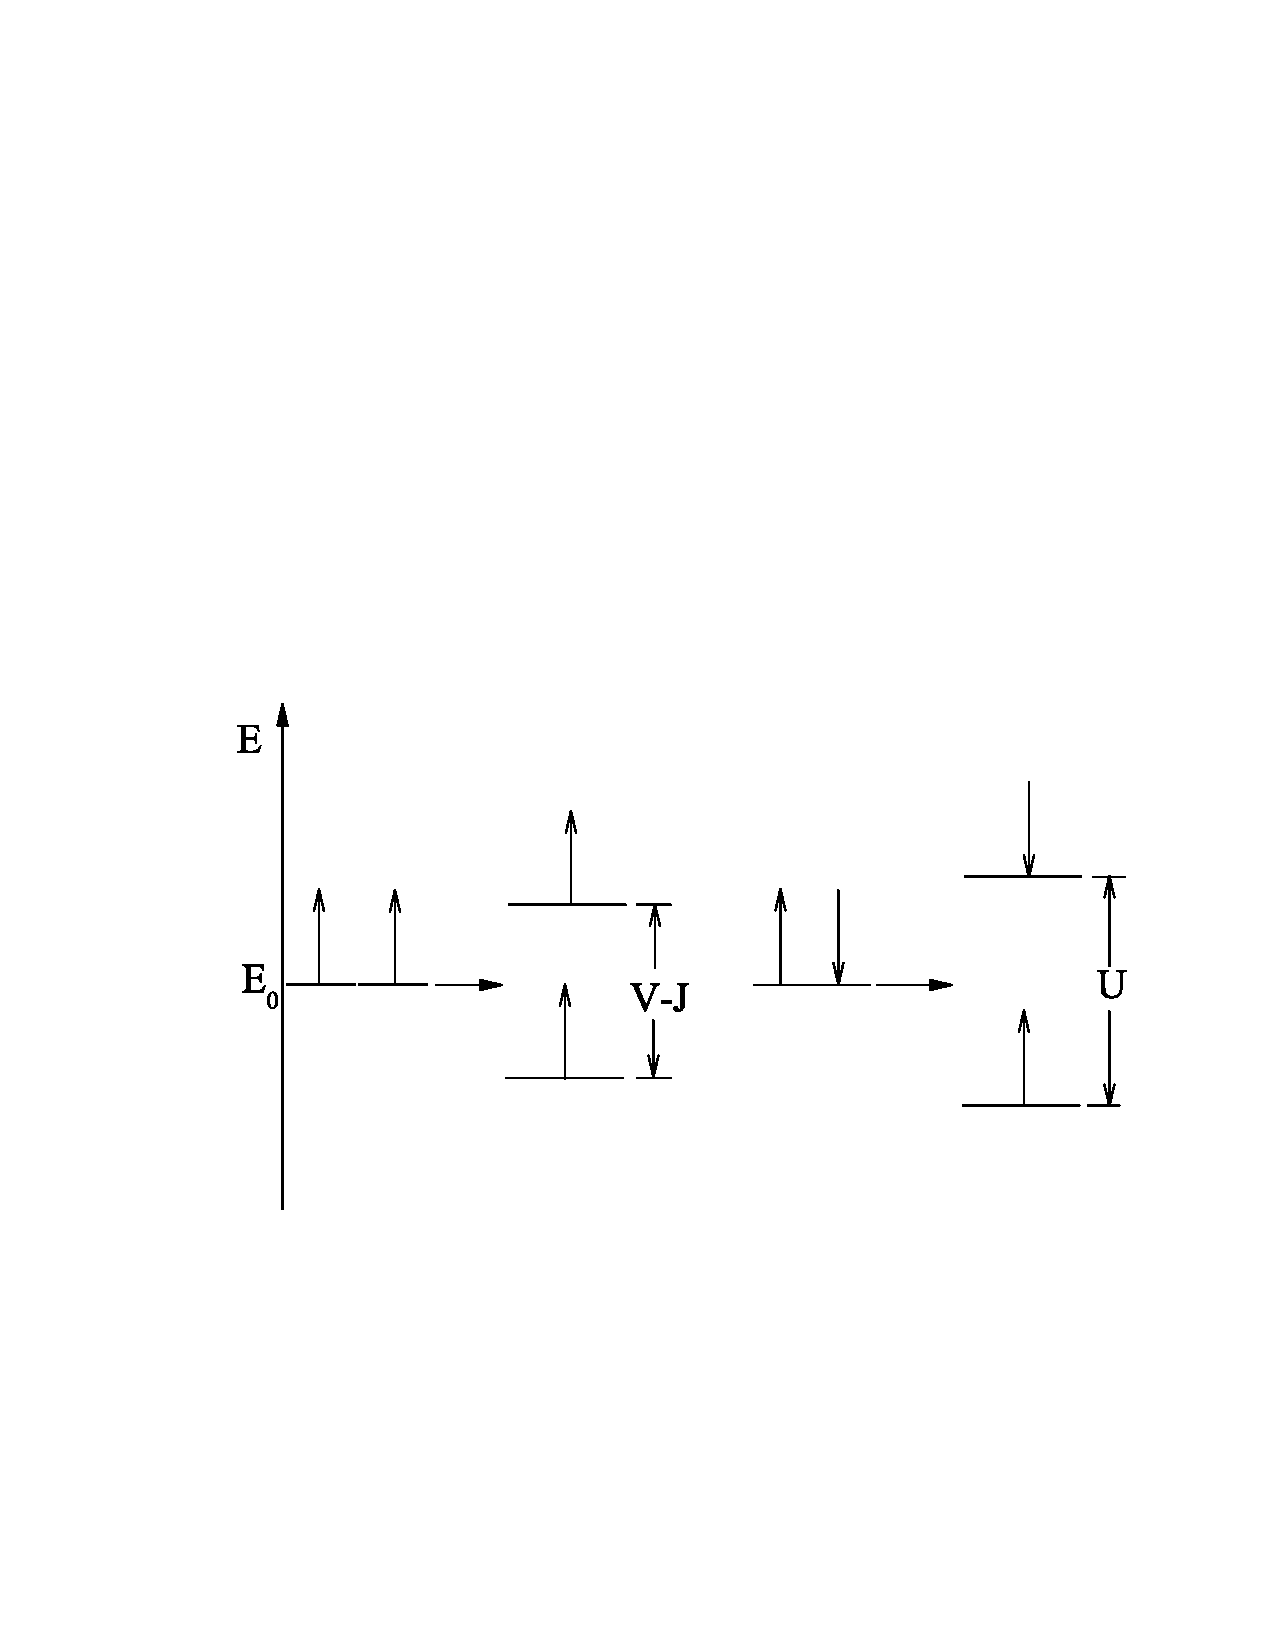
\includegraphics[height=1.35in,width=2.32in,viewport=110 210 545 455,clip]{LDA_U.pdf}
\caption{\small \textrm{The meaning of $U$, when the Coulomb-interaction of each electron is taken into account.}}%(与文献\cite{EPJB33-47_2003}图1对比)
\label{Tetrahedron_weight}
\end{figure}
该式将占据态轨道($n_i$=1)和非占据态轨道($n_i$=0)的LDA轨道能分别移动-$U$/2和+$U$/2,由此得到的轨道相关势[$V_i(\vec r)=\delta E/\delta n_i(\vec r)$]为
\begin{equation}
  V_i(\vec r)=V_{LDA}(\vec r)+U(\frac12-n_i)
  \label{eq:solid-253}
\end{equation}
式\eqref{eq:solid-253}表明\textrm{LDA}+$U$,通过简单引入唯象参数$U$,保留了精确密度泛函理论的单电子势能所必需的不连续特征。

式\eqref{eq:solid-251}没有考虑相同自旋电子的交换作用。设自旋$\sigma$的{\textit d}-{\textit d}\,电子间交换参数为{\textit J}\,,则{\textit N}\,电子的LDA近似下{\textit d}-{\textit d}\,相互作用为$UN(N-1)/2-JN(N-2)/4$。

如果进一步考虑Coulomb势和交换势的非球形部分的贡献(与{\textit d}\,轨道的$m$和$m^{\prime}$相关部分),引入矩阵元$U_{mm^{\prime}}$和$J_{mm^{\prime}}$,有
\begin{equation}
  U_{mm^{\prime}}=\sum_ka_kF^k
  \label{eq:solid-210}
\end{equation}
\begin{equation}
  J_{mm^{\prime}}=\sum_kb_kJ^k
  \label{eq:solid-211}
\end{equation}
\begin{equation}
  a_k=\frac{4\pi}{2k+1}\sum_{q=-k}^k\langle lm|Y_{kq}|lm\rangle\langle lm|Y_{kq}^{\ast}|lm^{\prime}\rangle
  \label{eq:solid-212}
\end{equation}
\begin{equation}
  b_k=\frac{4\pi}{2k+1}\sum_{q=-k}^k|\langle lm|Y_{kq}|lm^{\prime}\rangle|^2
  \label{eq:solid-213}
\end{equation}
这里$F^k$是Slater积分,$\langle lm|Y_{kq}|lm^{\prime}\rangle$是三个球谐函数$Y_{lm}$的乘积的积分。

由此得到的总能量为
\begin{equation}
  \begin{split}
	  E=&E_{\mathrm{LDA}}-[UN(N-1)/2-JN(N-2)/4]\\
  &+\frac12\sum_{m,m^{\prime},\sigma}U_{mm^{\prime}}n_{m\sigma}n_{m^{\prime}\sigma}\\
  &+\frac12\sum_{m\neq m^{\prime},m^{\prime},\sigma}(U_{mm^{\prime}}-J_{mm^{\prime}})n_{m\sigma}n_{m^{\prime}\sigma}
  \end{split}
  \label{eq:solid-214}
\end{equation}
式\eqref{eq:solid-214}应占据数$n_{m\sigma}$求导,得到轨道相关的单电子势能
\begin{equation}
  \begin{split}
	  V_{m\sigma}(\vec r)=&V_{\mathrm{LDA}}(\vec r)+\sum_{m^{\prime}}(U_{mm^{\prime}}-U_{\mathrm{eff}})n_{m-\sigma}\\
	  &\sum_{m\neq m^{\prime}}(U_{mm^{\prime}}-J{mm^{\prime}}-U_{\mathrm{eff}})n_{m\sigma}+U_{eff}\left(\frac12-n_{m\sigma}\right)-\frac12J
  \end{split}
  \label{eq:solid-215}
\end{equation}
这里$U_{\mathrm{eff}}=U-J/2$。

为了计算矩阵元$U_{mm^{\prime}}$和$J_{mm^{\prime}}$,必须知道Slater积分$F^k$(对{\it d}\,电子是$F^0$,$F^2$和$F^4$)。文献\cite{PRB43-7570_1991}用超晶胞近似(supercell approximation)给出Coulomb参数$U$,和$F^0$相等,将矩阵元$U_{mm^{\prime}}$和$(U_{mm^{\prime}}-J_{mm^{\prime}})$对所有$mm^{\prime}$求平均,可以得到$U$和$(U-J)$,根据Clebsch-Gordan系数性质,有平均值为
\begin{equation}
  U=\frac1{(2l+1)^2}\sum_{mm^{\prime}}U_{mm^{\prime}}=F^0
  \label{eq:solid-216}
\end{equation}
\begin{equation}
  U-J=\frac1{2l(2l+1)}\sum_{mm^{\prime}}(U_{mm^{\prime}}-J_{mm^{\prime}})=F^0-(F^2+F^4)
  \label{eq:solid-217}
\end{equation}
\begin{equation}
  J=(F^2=F^4)/4
  \label{eq:solid-218}
\end{equation}
为了由$U$和$J$得到所有的Slater积分,只需要知道$F^4/F^2$\cite{PRB42-5459_1990}。

LDA+$U$方法最重要的特征是具备了单电子势的不连续性。计算表明LDA+$U$方法对含有定域强Coulomb相互作用的体系是可靠的\cite{PRB48-16929_1993,JPCS56-1521_1995,EPL36-551_1996}。无论对含有近芯层的局域4{\textit f}\,电子的稀土金属离子还是对过渡金属的氧化物(金属的3{\textit d}\,电子与氧原子2{\textit p}\,轨道有很强的相互作用)体系都有效。尽管LDA+$U$方法只是通过参数$U$唯象地考虑电子间的关联效应,并未突破平均场近似框架,因此不足以描述金属-绝缘体的\textrm{Mott}转变和具有强关联的金属。但对诸如FeSi和LaCaO$_3$这类化合物,LDA+$U$已经能够给出有关于金属-绝缘体转变的有用信息\cite{JPCM9-767_1997}。甚至对含有5{\textit f}\,电子的化合物的研究也取得一定的成功\cite{PRB54-R3706_1996}。

\section{电子激发与GW近似}
Landau的Fermi液体理论是研究群体激发和多体Fermi子体系物理性质的重要方法\cite{Landau}。Fermi液体的特征是准粒子分布$\varepsilon=\varepsilon(\vec k)$由体系总能量$E$对分布函数的变分,即
\begin{equation}
  \frac{\delta E}{\delta n(\vec k)}=\varepsilon(\vec k)
  \label{eq:solid-219}
\end{equation}
关联函数$f(\vec k,\vec k^{\prime})$由准粒子能量对整个$\vec k$空间粒子分布变分得到
\begin{equation}
  \frac{\delta\varepsilon(\vec k)}{\delta n(\vec k^{\prime})}=\frac{\delta^2E}{\delta n(\vec k)\delta n(\vec k^{\prime})}=f(\vec k,\vec k^{\prime})
  \label{eq:solid-220}
\end{equation}
考虑准粒子间相互作用,体系激发能记作
\begin{equation}
  W=\sum_{\vec k}\varepsilon(\vec k)\delta n(\vec k)+\frac12\sum_{\vec k}\sum_{\vec k^{\prime}}f(\vec k,\vec k^{\prime})\delta n(\vec k)\delta(\vec k^{\prime})
  \label{eq:solid-221}
\end{equation}

Green函数是研究Fermi液体的重要数学工具。对宏观体系,Green函数定义为\cite{Lifshitz}
\begin{equation}
	\tilde G(x,x^{\prime})=-\mathrm{i}\langle T\hat\Psi(x)\hat\Psi^{\ast}(x^{\prime})\rangle
  \label{eq:solid-222}
\end{equation}
这里$x$表示时间$t$和位置$\vec r$,$\langle\cdots\rangle$表示对体系基态求平均,$T$表示按时间先后乘积算符。$\hat\Psi$是Heisenberg算符,对式\eqref{eq:solid-222}进行Fourier变换,得到以$\vec r$,$E$为表象的Green函数$\tilde G(\vec r,\vec r^{\prime};E)$是Dyson方程\cite{Lifshitz}
\begin{equation}
	(\dfrac12\nabla^2+E)\tilde G(\vec r,\vec r^{\prime};E)-\int\mathrm{d}\vec r^{\prime\prime}\Sigma(\vec r,\vec r^{\prime\prime};E)\tilde G(\vec r^{\prime\prime},\vec r^{\prime};E)=\delta(\vec r-\vec r^{\prime})
  \label{eq:solid-223}
\end{equation}
的解。这里$\Sigma(\vec r,\vec r^{\prime};E)$是描述交换和相关效应的质量或自能算符,这是个与能量有关的非定域的非-Hermitian算符,考虑到粒子与体系中其他粒子的相互作用。晶体中的质量具有平移对称性,
\begin{equation}
  \Sigma(\vec r+\vec a,\vec r+\vec a;E)=\Sigma(\vec r,\vec r^{\prime};E),
  \label{eq:solid:224}
\end{equation}
这里$\vec a$是晶体平移格矢。

临近Green函数的极点,式\eqref{eq:solid-223}右面的$\delta$函数为0,所得积分-微分方程的本征值确定体系激发能谱\cite{Lifshitz,PR145-561_1966}
\begin{equation}
	-\delta^2\Phi_{\vec k}(\vec r,E)+\int\mathrm{d}\vec r^{\prime}\Sigma(\vec r,\vec r^{\prime};E)\Phi_{\vec k}(\vec r^{\prime},E)=\varepsilon_{\vec k}\Phi_{\vec k}(\vec r,E) 
  \label{eq:solid-225}
\end{equation}
这里函数$\Phi_{\vec k}(\vec r,E)$类似于周期场中的单电子Bloch波函数。对金属中的Fermi电子液体中用式\eqref{eq:solid-225}替代一般Schr\"odinger方程。与一般的Schr\"odinger方程不同,式\eqref{eq:solid-225}的能量本征值是复数,因为质量算符$\Sigma(\vec r,\vec r^{\prime};E)$是复数。

由式(\ref{eq:solid-223},\ref{eq:solid-225})得到Green函数
\begin{equation}
	\tilde G(\vec r,\vec r^{\prime};E)=\sum_{\vec k}\frac{\Phi_{\vec k}(\vec r,E)\Phi_{\vec k}^{\ast}(\vec r^{\prime},E)}{E-\varepsilon_{\vec k}(E)+\mathrm{i}0\mathrm{sgn}E}
  \label{eq:solid-226}
\end{equation}
$\varepsilon_{\vec k}(E)$是体系中加入一个粒子引起的能量改变。如果将单个准粒子改变引起得能量变化$\varepsilon_{\vec k}(E)$定义为式\eqref{eq:solid-219}中的准粒子能量,对临近Fermi面的态,函数$\tilde G(\vec r,\vec r^{\prime};E)$在$E=\varepsilon_{\vec k}(E)$有极值。因此Green函数极值确定了多Fermi子体系的元激发能谱。一般说,因为和其他粒子相互作用,准粒子能量为复数。复数能量使得体系激发态的寿命有限$(\tau\sim1/|\mathrm{Im}\varepsilon|)$\cite{Landau-Lifshitz}。能量宽度由$\mathrm{Im}\varepsilon$确定。

%临近Fermi能级,$\mathrm{Im}\varepsilon_{\vec k}(E)\rightarrow0$,相应的$\mathrm{Im}\Sigma\rightarrow0$,于是解方程\eqref{eq:solid-225}得到$\mathrm{Re}\varepsilon_{\vec k}(E)$和实数形式的$\Sigma(\vec r,\vec r^{\prime};E)$和$\epsilon_{\vec k}(E)$。

根据Hohenberg-Kohn定理,本征值$\Sigma(\vec r,\vec r^{\prime};E)$由体系基态确定,它也是电子密度的函数。Sham和Kohn建议可用局域电子密度近似表示$\Sigma(\vec r,\vec r^{\prime};E)$\cite{PR145-561_1966}:
\begin{equation}
  \Sigma(\vec r,\vec r^{\prime};E)=V_C(\vec r)\delta(\vec r-\vec r^{\prime})+\Sigma_0(\vec r-\vec r^{\prime};E-V_C(\vec r_0);\rho(\vec r_0))
  \label{eq:solid-227}
\end{equation}
这里$\Sigma_0$是密度为$\rho$的无相互作用电子气的本征能量,$V_C(\vec r_0)$是位于$\vec r_0=(\vec r+\vec r^{\prime})/2$的静电Coulomb势。此外式\eqref{eq:solid-227}已将能量$\Sigma$中的局域部分以Hartree势的形式分离出来,因此可以利用$\Sigma_0$的短程效应。

对本征函数$\Phi_{\vec k}$作近似
$$\Phi_{\vec k}(\vec r,E)=A(\vec k)\exp[\mathrm{i}\vec p(\vec r)\vec r]$$
并认为$A$和电子动量与$\vec r$无关,将式\eqref{eq:solid-225}称为类似Kohn-Sham方程的表达式\cite{JPC4-2064_1971},
\begin{equation}
  [-\dfrac12\nabla^2+V_C(\vec r)+\Sigma_{xc}(\rho(\vec r),E)]\Phi_{\vec k}(\vec r,E)=\varepsilon_{\vec k}(\vec r,E)
  \label{eq:solid-228}
\end{equation}
若$E=\mu$,$\Sigma_{xc}(\rho(\vec r),\mu)\equiv\mu_{xc}(\rho(\vec r))$我们因此得到符合局域密度近似的DFT方程,两者的交换-相关势$\mu_{xc}$是相同的。因此对于低激发能,可以使用近似$\Sigma_{xc}(\rho(\vec r),E)\simeq\mu_{xc}$,此结果对应于忽略准粒子间的相互作用,即Landau函数$f(\vec k,\vec k^{\prime})=0$。

因此基于DFT的能带计算,如果充分考虑交换-相关效应,可以计算多电子体系的元激发能量。注意,采用单电子近似,要求能带比较宽,即中心位于不同格点的波函数有较大的重叠,电子间相互作用不是很强。

Hedin和Lundqvist详细回顾了用Green函数技术解决电子相关的问题\cite{Hedin-Lundqvist}。在单粒子近似下的Green函数,准粒子与谱函数的峰联系在一起。如果峰足够尖锐,表明存在一个明确的准粒子能量,对一般的非均匀体系,准粒子能量和波函数可以通过解Dyson方程\eqref{eq:solid-225}求得。对于准粒子问题,核心问题是对自能算符$\Sigma(\vec r,\vec r^{\prime};E)$的足够好的近似。常用的方法是GW近似\cite{PR139-A796_1965},自能用屏蔽相互作用$W$计算到最低阶。
\begin{equation}
	\Sigma(\vec r,\vec r^{\prime};E)=\dfrac{\mathrm{i}}{2\pi}\int_{-\infty}^{\infty}\mathrm{d}E^{\prime}\tilde G(\vec r,\vec r^{\prime};E+E^{\prime})W(\vec r,\vec r^{\prime};E^{\prime})
  \label{eq:solid-229}
\end{equation}
Green函数$\tilde G$由准粒子的波函数和能量表示,屏蔽Coulomb作用$W$
\begin{equation}
	W(\vec r,\vec r^{\prime};E)=\frac1{\Omega}\int\mathrm{d}^3r^{\prime\prime}\varepsilon^{-1}(\vec r,\vec r^{\prime\prime};E)V(\vec r^{\prime\prime}-\vec r^{\prime})
  \label{eq:solid-230}
\end{equation}
这里$V$是未屏蔽的Coulomb势,$\varepsilon^{-1}$是介电函数矩阵的逆阵,
\begin{equation}
	\varepsilon^{-1}(\vec r,\vec r^{\prime};E)=\delta(\vec r-\vec r^{\prime})+\int\mathrm{d}^3r^{\prime\prime}V(\vec r^{\prime}-\vec r^{\prime\prime})P(\vec r^{\prime\prime},\vec r^{\prime};E)
  \label{eq:solid-231}
\end{equation}
这里$P$是完全响应函数,于是
\begin{equation}
  W(\vec r,\vec r^{\prime};E)=V(\vec r-\vec r^{\prime})+W_c(\vec r,\vec r^{\prime};E)
  \label{eq:solid-232}
\end{equation}
这里
\begin{equation}
	W_c(\vec r,\vec r;E)=\int\mathrm{d}^3r_1d^3r_2V(\vec r^{\prime}-\vec r_1)P(\vec r_1,\vec r_2;E)V(\vec r_2-\vec r^{\prime})
  \label{eq:solid-233}
\end{equation}
Green函数可以写成谱表示
\begin{equation}
	G(\vec r,\vec r^{\prime};E)=\int_{-\infty}^{\mu}\mathrm{d}E^{\prime}\frac{A(\vec r,\vec r^{\prime};E^{\prime})}{E-E^{\prime}-i\delta}+\int_{\mu}^{\infty}\mathrm{d}E^{\prime}\frac{A(\vec r,\vec r^{\prime};E^{\prime})}{E-E^{\prime}+i\delta}
  \label{eq:solid-234}
\end{equation}
这里$A(\vec r,\vec r^{\prime};E)=-\frac1{\pi}\mathrm{Im}G(\vec r,\vec r^{\prime};E)\mathrm{sgn}(E-\mu)$

实际计算中,取零阶Green函数,有
\begin{equation}
  A(\vec r,\vec r^{\prime};E)=\sum_{kn}\psi_{kn}(\vec r)\psi_{kn}^{\ast}(\vec r^{\prime})\delta(E-E_{kn})
  \label{eq:solid-235}
\end{equation}
于是自能可以写成
\begin{equation}
  \Sigma(\vec r,\vec r^{\prime};E)=\Sigma_x(\vec r,\vec r^{\prime})+\Sigma_c(\vec r,\vec r^{\prime};E)
  \label{eq:solid-236}
\end{equation}
这里$\Sigma_x$是净的交换势,
\begin{equation}
	\Sigma_x(\vec r,\vec r^{\prime})=-\sum_{kn}^{\mathrm{occ}}\psi_{kn}(\vec r)\psi_{kn}^{\ast}(\vec r^{\prime})V(\vec r-\vec r^{\prime})
  \label{eq:solid-254}
\end{equation}
$E_c$自能的相关部分,
\begin{equation}
  \begin{split}
	  \Sigma_c(\vec r,\vec r^{\prime};E)=&\sum_{kn}^{\mathrm{occ}}\psi_{kn}(\vec r)\psi_{kn}^{\ast}(\vec r^{\prime})W_c^-(\vec r,\vec r^{\prime};E-E_{kn})\\
	  &+\sum_{kn}^{\mathrm{occ}}\psi_{kn}(\vec r)\psi_{\vec r}^{\ast}(\vec r^{\prime})W_c^+(\vec r,\vec r^{\prime};E-E_{kn})
  \end{split}
  \label{eq:solid-237}
\end{equation}
其中$W_c^{\pm}(\vec r,\vec r^{\prime};E)=\dfrac{\mathrm{i}}{2\pi}\int_{-\infty}^{+\infty}\mathrm{d}E^{\prime}\frac{W_c(\vec r,\vec r^{\prime};E^{\prime})}{E+E^{\prime}\pm i\delta}$。于是$\Sigma(\vec r,\vec r^{\prime};E)$可以记作\cite{JPCM9-767_1997},
\begin{displaymath}
  \Sigma(\vec r,\vec r^{\prime};E)=-\sum_{kn}\psi_{kn}(\vec r)\psi_{kn}^{\ast}(\vec r^{\prime})W_0(\vec r,\vec r^{\prime};E-E_{kn})
\end{displaymath}
其中
\begin{displaymath}
  \begin{aligned}
    W_0(\vec r,\vec r^{\prime};E-E_{kn})\equiv&[V(\vec r-\vec r^{\prime})-W_c^-(\vec r,\vec r^{\prime};E-E_{kn})]\theta(\mu-E_{kn})\\
    &-W_c^+(\vec r,\vec r^{\prime};E-E_{kn})\theta(E_{kn}-\mu)
  \end{aligned}
\end{displaymath}
这样的GWA近似的自能与Hartree-Fock方法具有相同的形式,但是自能是能量的函数且因为包含相关作用,因此也依赖于未占据态。GWA可以看作是包含动态屏蔽Coulomb势$W_0$的推广Hartree-Fock方法,注意这里的$W_0$与动态屏蔽势$W$不同。

在各种能带计算方法中引入GW近似,包括赝势方法\cite{PRB34-5390_1986},LMTO-TB方法\cite{PRL74-3221_1995}。GWA校正主要应用于简单金属和过渡金属体系,但由于计算过程比较复杂所以目前还没有广泛应用到复杂体系的计算中。GWA校正的另一个问题是计算屏蔽相互作用所需的响应函数,要借助LDA得到的波函数和能带来计算得到\cite{JPCM9-767_1997}。但是这样的方法只适用于电子相关较小的体系(比如绝缘体或者半导体);对电子强相关体系,则需要采用比LDA近似更好的Hamiltonian,一般可以通过自洽迭代来计算自能\cite{PRL74-3221_1995}。

\section{LDA+$U$和GWA校正的关系}
尽管GWA是由多体微扰理论导出的最简单的自能近似,但是计算量已经很大。GWA和LDA+$U$可以分别看作包含依赖于频率和轨道屏蔽Coulomb作用的Hartree-Fock方法。至少对含有局域的{\textit d}\,或{\textit f}\,轨道的过渡金属和稀土金属离子,LDA+$U$可以看作是对GWA的近似\cite{JPCM9-767_1997}。

LDA+$U$是针对包含在离域态中的定域态轨道的自能校正,定域态的强Coulomb相关用参数$U$校正,而离域态可以用LDA很好的描述。为了确定LDA+$U$和GWA之间的关系,对态$\psi_d$,考虑GWA中自能的相关部分
\begin{equation}
  \begin{split}
    \langle\psi_d|\Sigma_c(E_d)|\psi_d\rangle=&\langle\psi_d\psi_d|W_c^-|\psi_d\psi_d\rangle\\
    &+\sum_{kn\neq d}^{\mathrm{occ}}\langle\psi_d\psi_{kn}|W_c^-(E_d-E_{kn})|\psi_{kn}\psi_d\rangle\\
    &+\sum_{kn}^{\mathrm{unocc}}\langle\psi_d\psi_{kn}|W_c^+(E_d-E_{kn})|\psi_{kn}\psi_d\rangle
  \end{split}
  \label{eq:solid-238}
\end{equation}
严格地说,自能应该是$\tilde E_d=E_d+$自能校正。如果$\psi_d$是局域的而且能量与其他态很好的分离,则式\eqref{eq:solid-238}第一项比剩下的其余项大得多,最后一项含未占据的$\psi_d$态,但因为这些项与占据态正交,因此这一项比第一项小得多。可作近似\cite{JPCM9-767_1997}
\begin{equation}
  \langle\psi_d|\Sigma_c(E_d)|\psi_d\rangle\approx\langle\psi_d\psi_d|W_c^-(0)|\psi_d\psi_d\rangle=-\frac12\langle\psi_d\psi_d|W_c(0)|\psi_d\psi_d\rangle
  \label{eq:solid-239}
\end{equation}
将屏蔽势关联部分写成谱函数表象,
\begin{equation}
	W_c(E)=\int_{-\infty}^0\mathrm{d}E^{\prime}\frac{B(E^{\prime})}{E-E^{\prime}-i\delta}+\int_0^{\infty}\mathrm{d}E^{\prime}\frac{B(E^{\prime})}{E-E^{\prime}+i\delta}
  \label{eq:solid-240}
\end{equation}
这里$B(E)=-\dfrac1{\pi}W_c(E)\mathrm{sgn}(E)$。
$W_c$是$E$的偶函数,因此$B(E)$是奇函数,因此$W_c^-(0)=-1/2W_c(0)$,类似的对未占据的{\textit d}\,态,有$+1/2\langle\psi_d\psi_d|W_c(0)|\psi_d\psi_d\rangle$,因此能量差为
\begin{equation}
  \begin{split}
	  \Delta&=E_2^{\mathrm{HF}}-E_1^{\mathrm{HF}}+\langle\psi_d\psi_d|W_c(0)|\psi_d\psi_d\rangle\\
    &=\langle\psi_d\psi_d|V|\psi_d\psi_d\rangle+\langle\psi_d\psi_d|W_c(0)|\psi_d\psi_d\rangle\\
    &=\langle\psi_d\psi_d|W(0)|\psi_d\psi_d\rangle
  \end{split}
  \label{eq:solid-241}
\end{equation}
这符合屏蔽Coulomb相互作用$\Delta=U\approx W(0)$。

上述近似中,局域态的GW自能为
\begin{equation}
  \Sigma(\vec r,\vec r^{\prime};E_d)=\Sigma_x(\vec r,\vec r^{\prime})+\sum_{kn=d}\psi(\vec r)\psi_{kn}^{\ast}(\vec r^{\prime})W_c^0(\vec r,\vec r^{\prime};E_d)
  \label{eq:solid-242}
\end{equation}
这里$$W_c^0(\vec r,\vec r^{\prime};E)=-\frac12W_c(\vec r,\vec r^{\prime};0)[\theta(\mu-E_d)-\theta(E_d-\mu)]$$
LDA的自能校正
\begin{equation}
  \Delta\Sigma(\vec r,\vec r^{\prime};E_d)=\Sigma(\vec r,\vec r^{\prime};E_d)-V_{xc}^{LDA}(\vec r)\delta(\vec r-\vec r^{\prime})
  \label{eq:solid-243}
\end{equation}
应该与LDA+$U$方法的$U$值相等。按照LDA+$U$思想,将空间分为定域部分$\phi_m$(一般是{\textit d}\,和{\textit f}\,态)和离域部分$\psi_{kn}$
$$\delta(\vec r-\vec r^{\prime})=\sum_m\phi_m(\vec r)\phi_m^{\ast}(\vec r^{\prime})+\sum_{kn}\psi_{kn}(\vec r)\psi_{kn}^{\ast}(\vec r^{\prime})$$
自能校正可以写成
\begin{equation}
  \begin{split}
    \Delta(\vec r,\vec r^{\prime};E_d)=&\sum_{mm^{\prime}}\phi_m(\vec r)\Delta\Sigma_{mm^{\prime}}(E_d)\phi_{m^{\prime}}^{\ast}(\vec r^{\prime})+\sum_{knn^{\prime}}\psi_{kn}(\vec r)\Delta\Sigma_{nn^{\prime}}(E_d)\psi_{kn}^{\ast}(\vec r^{\prime})\\
    &+\sum_{knm}\psi_{kn}(\vec r)\delta\Sigma_{nm}(\vec k,E_d)\phi_m^{\ast}(\vec r^{\prime})+\sum_{kmn}\phi_m(\vec r)\Delta\Sigma_{mn}(\vec k,E_d)\psi_{kn}^{\ast}(\vec r^{\prime})
  \end{split}
  \label{eq:solid-244}
\end{equation}
其中第一项是主要的,有近似
$$\Delta\Sigma(\vec r,\vec r;E_d)\approx\sum_{mm^{\prime}}\phi_m(\vec r)\Delta\Sigma_{mm^{\prime}}(E_d)\phi_{m^{\prime}}^{\ast}(\vec r^{\prime})$$
这里$$\Delta\Sigma_{mm^{\prime}}(E_d)=\langle\phi_m|\Sigma_x-V_{xc}|\phi_m\rangle+\sum_{m^{\prime}m^{\prime\prime}}\langle m,m^{\prime\prime}|W_c^0|m^{\prime\prime\prime},m^{\prime}\rangle n_{m^{\prime\prime},m^{\prime\prime\prime}}$$
这里$$n_{m^{\prime\prime},m^{\prime\prime\prime}}=\sum_{kn=d}\langle\phi_{m^{\prime\prime}}|\psi_{kn}\rangle\langle\psi_{kn}|\phi_{m^{\prime\prime\prime}}\rangle$$
注意到选择的$\phi_m$是原子内的局域轨道,剩下的自能很小,可以包含在单电子项中。

假设只有一个{\it d}\,轨道$\psi_{m\sigma}$的{\it d}\,离子,根据上述近似,局域态的GWA自能为
\begin{equation}
  \Sigma(\vec r,\vec r^{\prime};E_{m\sigma})=\Sigma_x(\vec r,\vec r^{\prime})+\sum_{m^{\prime}\omega^{\prime}}\psi_{m^{\prime}\omega^{\prime}}(\vec r)\psi_{m^{\prime}\sigma^{\prime}}^{\ast}(\vec r^{\prime})W_c^0(\vec r,\vec r^{\prime};E_{m\sigma})
  \label{eq:solid-245}
\end{equation}
这里$$W_c^0(\vec r,\vec r^{\prime};E_{m\sigma})=-\frac12W_c(\vec r,\vec r^{\prime};0)[\theta(\mu-E_{m\omega})-\theta(E_{m\sigma}-\mu)]$$
GWA中的电子-电子相互作用的总势能的矩阵元可以写成
\begin{equation}
  \begin{split}
	  \langle\psi_{m\sigma}&|V_{\mathrm{H}}+\Sigma_x+\Sigma_c|\psi_{m\sigma}\rangle\\
	  =&\sum_{m^{\prime}\sigma^{\prime}}^{\mathrm{occ}}\iint\mathrm{d}\vec rd\vec r^{\prime}\psi_{m\omega}^{\ast}(\vec r)\psi_{m\omega}(\vec r)V(\vec r-\vec r^{\prime})\psi_{m^{\prime}\sigma^{\prime}}^{\ast}(\vec r^{\prime})\psi_{m^{\prime}\sigma^{\prime}}(\vec r^{\prime})\\
	  &-\sum_{m^{\prime}}^{\mathrm{occ}}\iint\mathrm{d}\vec rd\vec r^{\prime}\psi_{m\omega}^{\ast}(\vec r)\psi_{m^{\prime}\omega^{\prime}}(\vec r)V(\vec r-\vec r^{\prime})\psi_{m\sigma}^{\ast}(\vec r^{\prime})\psi_{m^{\prime}\sigma^{\prime}}(\vec r^{\prime})\\
    &+\left(\frac12-n_{m\sigma}\right)\sum_{m^{\prime}}\iint\mathrm{d}\vec rd\vec r^{\prime}\psi_{m\omega}^{\ast}(\vec r)\psi_{m^{\prime}\omega^{\prime}}(\vec r)W_c(\vec r,\vec r^{\prime};0)\psi_{m\sigma}^{\ast}(\vec r^{\prime})\psi_{m^{\prime}\sigma^{\prime}}(\vec r^{\prime})
  \end{split}
  \label{eq:solid-246}
\end{equation}
这里$n_{m\sigma}$是$m\sigma$轨道占据状态,如$\mu-E_{m\sigma}>0$则$n_{m\sigma}=1$;$\mu-E_{m\sigma}<0$,有$n_{m\sigma}=0$。上述矩阵元可以写成
$$V_{m\sigma}^{\mathrm{GWA}}=\sum_{m^{\prime}\sigma^{\prime}}U_{mm^{\prime}}^0n_{m^{\prime}\sigma^{\prime}}-U_{mm}^0n_{m\sigma}-\sum_{m^{\prime}\neq m}J_{mm^{\prime}}n_{m^{\prime}\sigma}+\left(\frac12-n_{m\sigma}\right)\sum_{m^{\prime}}W_{mm^{\prime}}$$
这里$U_{mm^{\prime}}^0$是未屏蔽的Coulomb相互作用矩阵元。$J_{mm^{\prime}}$是交换矩阵,$W_{mm^{\prime}}$是交换势$W_c(\vec r,\vec r^{\prime};0)$矩阵元。将屏蔽参数定义为$W=-\sum\limits_{m^{\prime}}W_{mm^{\prime}}$,最终GWA的势能矩阵元表达式为\cite{JPCM9-767_1997}
\begin{equation}
	V_{m\sigma}^{\mathrm{GWA}}=\sum_{m^{\prime}\sigma^{\prime}}U_{mm^{\prime}}^0n_{m^{\prime}\sigma^{\prime}}-(U_{mm}^0-W)n_{m\sigma}-\sum_{m^{\prime}\neq m}J_{mm^{\prime}}n_{m^{\prime}\sigma}-\frac12W
  \label{eq:solid-247}
\end{equation}
为了将LDA的校正写成GWA形式,必须将LSDA的势能矩阵元写成上述相似的形式,因为LSDA并非由轨道-轨道相互作用导出,而由类似于均匀电子气的处理方式,用与Coulomb相互作用能有关的电荷密度计算得到的与轨道无关的有效局域势,无法严格处理。{\textit d}\,电子的相互作用能作为总的{\textit d}\,电子数$N$的函数,$E_{\mathrm{LSDA}}[\rho(\vec r)]=E_{\mathrm{LSDA}}[N|\psi_{m\sigma}(\vec r)|^2]$。已知LSDA中单电子本征能不是很准确,但是总能量比较准确,于是假设Hartree-Fock计算是好的近似
\begin{equation}
  \begin{split}
	  E_{\mathrm{LSDA}}[\rho_{\sigma}(\vec r)]&=E_{\mathrm{LSDA}}[N_{\sigma}|\psi_{m\sigma}(\vec r)|^2]\\
   &=\frac12F^0N(N-1)-\frac14JN(N-2)\frac14J(N_{\uparrow}-N_{\downarrow})^2
 \end{split}
  \label{eq:solid-248}
\end{equation}
这里$F^0$是第一Slater积分,$J$是交换能参数,$N_{\sigma}=\sum\nolimits_mn_{m\sigma}$,$N=N_{\uparrow}+N_{\downarrow}$

LSDA的电子相互作用势能是总能量对电荷密度$\rho(\vec r)$的变分导数,相互作用能作为总的{\it d}\,电子总数$N_{\sigma}$的变分导数为:
\begin{equation}
  \begin{split}
	  \frac{\partial E_{\mathrm{LSDA}}[N_{\sigma}|\psi_{m\sigma}(\vec r)|^2]}{\partial N_{\sigma}}&=\int\mathrm{d}\vec r\frac{\delta E_{\mathrm{LSDA}}[\rho(\vec r)]}{\delta\rho_{\sigma}(\vec r)}\frac{\partial\rho_{\sigma}(\vec r)}{\partial N_{\sigma}}\\
	  &=\int\mathrm{d}\vec rV_{\mathrm{LSDA}}^{\sigma}(\rho(\vec r))|\psi_{m\sigma}(\vec r)|^2\\
    &=F^0N-\frac12(F^0-J)-JN_{\sigma}
  \end{split}
  \label{eq:solid-257}
\end{equation}
由此可有LSDA的势能矩阵元为$V_{m\sigma}^{\mathrm{LSDA}}=F^0N-\frac12(F^0-J)-JN_{\sigma}$。
GWA对LSDA的势能校正为\cite{JPCM9-767_1997}
\begin{equation}
  \begin{split}
	  \delta V_{m\sigma}=&V_{m\sigma}^{\mathrm{GWA}}-V_{m\sigma}^{\mathrm{LSDA}}\\
    =&\sum_{m^{\prime}\sigma^{\prime}}U_{mm^{\prime}}^0n_{m^{\prime}\sigma^{\prime}}-(U_{mm}^0-W)n_{m\sigma}-\sum_{m^{\prime}\neq m}j_{mm^{\prime}}n_{m^{\prime}\sigma}-\frac12W\\
    &-F^0\sum_{m^{\prime}\sigma^{\prime}}n_{m^{\prime}\sigma^{\prime}}+J\sum_mn_{m\sigma}+\frac12(F^0-J)\\
    =&\sum_{m^{\prime}\sigma^{\prime}}(U_{mm^{\prime}}^0-F^0)n_{m^{\prime}\sigma^{\prime}}-(U_{mm}^0-W)n_{m\sigma}-\sum_{m^{\prime}\neq m}j_{mm^{\prime}}n_{m^{\prime}\sigma}\\
    &-\frac12W+J\sum_mn_{n\sigma}+\frac12(F^0-J)
  \end{split}
  \label{eq:solid-249}
\end{equation}
差值$U_{mm^{\prime}}^0-F^0$与Slater积分$F^0$无关(只与Slater积分$F^k$且$k\neq0$有关),而且有$U_{mm^{\prime}}^0-F^0=U_{mm^{\prime}}-U$,这里$U=F^0-W$是屏蔽Coulomb参数,$U_{mm^{\prime}}$是屏蔽Coulomb矩阵元。
\begin{equation}
  \begin{split}
	  \delta V_{m\sigma}=&V_{m\sigma}^{\mathrm{GWA}}-V_{m\sigma}^{\mathrm{LSDA}}\\
    =&\sum_{m^{\prime}}U_{mm^{\prime}}n_{m^{\prime}-\sigma}+\sum_{m^{\prime}\neq m}(U_{mm^{\prime}}-J_{mm^{\prime}})n_{m^{\prime}\sigma}\\
    &-U(N-\frac12)+J(N_{\sigma}-\frac12)
  \end{split}
  \label{eq:solid-250}
\end{equation}
如果占据矩阵是对角化的,式\eqref{eq:solid-250}等价于LDA+$U$势校正\eqref{eq:solid-215}。GWA和LDA+$U$的本质差别在于计算屏蔽Coulomb势参数$U$,在LDA+$U$中,$U$是通过构造LSDA超晶胞计算的,在GWA中则是通过计算响应函数得到的。
%\newpage
%\bibliographystyle{mythesis}
%%  \phantomsection\addcontentsline{toc}{section}{bibliography}
%  {\small\bibliography{bib/Myref}}
%%  \nocite{*}
